% Options for packages loaded elsewhere
\PassOptionsToPackage{unicode}{hyperref}
\PassOptionsToPackage{hyphens}{url}
\documentclass[
]{article}
\usepackage{xcolor}
\usepackage[margin=24mm]{geometry}
\usepackage{amsmath,amssymb}
\setcounter{secnumdepth}{-\maxdimen} % remove section numbering
\usepackage{iftex}
\ifPDFTeX
  \usepackage[T1]{fontenc}
  \usepackage[utf8]{inputenc}
  \usepackage{textcomp} % provide euro and other symbols
\else % if luatex or xetex
  \usepackage{unicode-math} % this also loads fontspec
  \defaultfontfeatures{Scale=MatchLowercase}
  \defaultfontfeatures[\rmfamily]{Ligatures=TeX,Scale=1}
\fi
\usepackage{lmodern}
\ifPDFTeX\else
  % xetex/luatex font selection
\fi
% Use upquote if available, for straight quotes in verbatim environments
\IfFileExists{upquote.sty}{\usepackage{upquote}}{}
\IfFileExists{microtype.sty}{% use microtype if available
  \usepackage[]{microtype}
  \UseMicrotypeSet[protrusion]{basicmath} % disable protrusion for tt fonts
}{}
\makeatletter
\@ifundefined{KOMAClassName}{% if non-KOMA class
  \IfFileExists{parskip.sty}{%
    \usepackage{parskip}
  }{% else
    \setlength{\parindent}{0pt}
    \setlength{\parskip}{6pt plus 2pt minus 1pt}}
}{% if KOMA class
  \KOMAoptions{parskip=half}}
\makeatother
\usepackage{graphicx}
\makeatletter
\newsavebox\pandoc@box
\newcommand*\pandocbounded[1]{% scales image to fit in text height/width
  \sbox\pandoc@box{#1}%
  \Gscale@div\@tempa{\textheight}{\dimexpr\ht\pandoc@box+\dp\pandoc@box\relax}%
  \Gscale@div\@tempb{\linewidth}{\wd\pandoc@box}%
  \ifdim\@tempb\p@<\@tempa\p@\let\@tempa\@tempb\fi% select the smaller of both
  \ifdim\@tempa\p@<\p@\scalebox{\@tempa}{\usebox\pandoc@box}%
  \else\usebox{\pandoc@box}%
  \fi%
}
% Set default figure placement to htbp
\def\fps@figure{htbp}
\makeatother
\setlength{\emergencystretch}{3em} % prevent overfull lines
\providecommand{\tightlist}{%
  \setlength{\itemsep}{0pt}\setlength{\parskip}{0pt}}
\usepackage{mathrsfs}
\usepackage{mathtools}
\DeclareUnicodeCharacter{2212}{\ensuremath{-}}

\DeclareUnicodeCharacter{2265}{\ensuremath{\ge}}
\DeclareUnicodeCharacter{2264}{\ensuremath{\le}}
\DeclareUnicodeCharacter{2295}{\ensuremath{\oplus}}
\DeclareUnicodeCharacter{2297}{\ensuremath{\otimes}}
\DeclareUnicodeCharacter{2208}{\ensuremath{\in}}
\DeclareUnicodeCharacter{2261}{\ensuremath{\equiv}}
\DeclareUnicodeCharacter{21A6}{\ensuremath{\mapsto}}
\DeclareUnicodeCharacter{2192}{\ensuremath{\to}}
\DeclareUnicodeCharacter{03BA}{\ensuremath{\kappa}}
\DeclareUnicodeCharacter{039B}{\ensuremath{\Lambda}}
\DeclareUnicodeCharacter{03C4}{\ensuremath{\tau}}
\DeclareUnicodeCharacter{03A9}{\ensuremath{\Omega}}
\usepackage{bookmark}
\IfFileExists{xurl.sty}{\usepackage{xurl}}{} % add URL line breaks if available
\urlstyle{same}
\hypersetup{
  hidelinks,
  pdfcreator={LaTeX via pandoc}}

\author{}
\date{}

\begin{document}

{
\setcounter{tocdepth}{3}
\tableofcontents
}
\section{Cotangent and Frobenius calculations for the observed
collision}\label{cotangent-and-frobenius-calculations-for-the-observed-collision}

This note retains the coefficients \[
a>0,\quad\varepsilon>0,\quad r\in\mathbb C,\quad
\lambda(s)=as+\varepsilon r,\quad s_*=-\varepsilon r/a.
\tag{OCF1}
\] They are fixed coefficients of the complex family. Set \[
B=\mathbb C[s],\quad P_0=B[z],\quad
f=z(z-\lambda),\quad A=P_0/(f),\quad
D=A/(s-s_*)=\mathbb C[z]/(z^2).
\tag{OCF2}
\] The scalar \(\varepsilon\), the polynomial \(z\), and the external
programme element \(\tau\) are different objects. The later integral
parameter \(\mathsf b\) is formal. It is not an asserted \(p\)-adic
value of \(\varepsilon r\), or of any area coefficient used elsewhere in
the reader.

The programme inputs are
\href{https://github.com/KokunoYumeto/zeta-function-research-reader/blob/6af54ea3c8ef99127af327f3103e086c68d482c2/workbenches/splitzero-tandem/branches/identity-absorber-square/NODE_COTANGENT.md}{Node
cotangent, N1--N8, N16--N24 and N28--N32} and
\href{https://github.com/KokunoYumeto/zeta-function-research-reader/blob/6af54ea3c8ef99127af327f3103e086c68d482c2/workbenches/splitzero-tandem/branches/identity-absorber-square/PRISMATIC_COMPARISON.md}{Prismatic
comparison, Theorems P1--P5}. The observed family is the public result
\href{https://github.com/KokunoYumeto/zeta-function-research-reader/blob/4ba9285b66af58a6d58fc502a494c1fb45ca5b79/workbenches/splitzero-tandem/continuations/20260922-support-transport/OBSERVED_DEFORMATION_AND_CURRENT.md\#L22}{DF1--12},
rederived with its full operator receiver in
\href{OBSERVED_COLLISION.md}{Observed collision}, OC1--OC17.

The regular-hypersurface cotangent formula used below is Luc Illusie's
regular-immersion theorem, \emph{Complexe cotangent et déformations}, I,
III Proposition 3.2.4(iii), combined with transitivity, II Proposition
2.1.2. Its exact source use is documented in the linked Node cotangent
note, Section 10. This task read the two specified programme notes; it
does not claim a new reading of Illusie's complete work. All
calculations for the observed coefficients are proved below.

\subsection{1. The full coordinate map and
flatness}\label{the-full-coordinate-map-and-flatness}

Monic division gives \[
A=B\oplus Bz,\qquad z^2=\lambda z.
\tag{OCF3}
\] Thus \(A\) is free of rank two, hence flat over \(B\): tensoring with
it is a direct sum of two copies of tensoring with \(B\). Also \(f\) is
a nonzerodivisor in the domain \(P_0\). Cancellation of \(f\) identifies
the conormal module \((f)/(f^2)\) with the free module \(A\overline f\).

The coordinate map and its inverse are \[
x=z,\quad y=z-as-\varepsilon r;
\qquad z=x,\quad s=\frac{x-y-\varepsilon r}{a}.
\tag{OCF4}
\] Both compositions fix every generator. The equation becomes exactly
\(f=xy\), so \[
A\cong\mathbb C[x,y]/(xy),\qquad
\lambda=x-y,\quad s-s_*=(x-y)/a.
\tag{OCF5}
\] No coefficient has been suppressed. In particular \[
dz=dx,\quad ds=(dx-dy)/a,\quad
df=(2z-\lambda)dz-az\,ds=y\,dx+x\,dy.
\tag{OCF6}
\]

The branch map \[
A\longrightarrow B\times B,\qquad
h(s,z)\longmapsto(h(s,0),h(s,\lambda))
\tag{OCF7}
\] is injective with image \(\{(u,v):v-u\in\lambda B\}\). Indeed
\(c+dz\) maps to \((c,c+d\lambda)\), which is zero only if \(c=d=0\);
conversely every such pair has that lift. Here \(\lambda\ne0\) in the
domain \(B\). Multiplication by \(\lambda\) in \(A\) is injective also
directly from (OCF3).

\subsection{2. Relative and absolute cotangent
complexes}\label{relative-and-absolute-cotangent-complexes}

All complexes here use cohomological degrees \(-1,0\). The hypersurface
formula applies: the ambient algebra is polynomial over the stated base
and its equation is a nonzerodivisor. It gives \[
L_{A/B}\simeq
[A\overline f\xrightarrow{\,2z-\lambda\,}A\,dz],
\tag{OCF8}
\] and \[
L_{A/\mathbb C}\simeq
[A\overline f\xrightarrow{\,(-az,\;2z-\lambda)\,}
 A\,ds\oplus A\,dz].
\tag{OCF9}
\] The degree-zero presentations also follow directly from derivations:
their values on the polynomial generators must annihilate \(df\), and
that is the only relation. The free conormal module was proved above;
the regular-immersion formula and transitivity give these full complexes
without assuming that the quotient is smooth.

In \(A\) one has \[
(2z-\lambda)^2=\lambda^2.
\tag{OCF10}
\] Since \(\lambda\) is a nonzerodivisor, \(2z-\lambda\) is a
nonzerodivisor. Both displayed differentials are therefore injective. In
particular \[
H^{-1}(L_{A/B})=H^{-1}(L_{A/\mathbb C})=0,
\qquad
\Omega^1_{A/B}=A/(2z-\lambda)\,dz.
\tag{OCF11}
\] Over \(\mathbb C\), \[
A/(2z-\lambda)\cong B/(\lambda^2),\qquad z\mapsto\lambda/2.
\tag{OCF12}
\] Indeed \(2z-\lambda=0\) forces this image, after which
\(f=-\lambda^2/4\). These maps are inverse since 2 and 4 are units. This
argument will not be used at the prime 2.

The coefficientwise map from (OCF9) to (OCF8) kills \(ds\), fixes
\(dz\), and fixes \(\overline f\). It is a surjective cochain map with
kernel \(A\,ds\) in degree zero. Thus it realizes the transitivity
triangle \[
A\,ds\longrightarrow L_{A/\mathbb C}
\longrightarrow L_{A/B}\longrightarrow A\,ds[1].
\tag{OCF13}
\] Dualizing (OCF9) further gives \[
\operatorname{Ext}^1_A(L_{A/\mathbb C},A)
=A/(az,2z-\lambda)=A/(z,\lambda)\cong\mathbb C.
\tag{OCF14}
\] The equality of the two ideals uses \(a\ne0\); setting \(z=0\) in the
second generator then gives \(-\lambda\).

\subsection{3. The discriminant and the two different collision
pullbacks}\label{the-discriminant-and-the-two-different-collision-pullbacks}

Multiplication by \(z\) in the original basis \(1,z\) has matrix \[
\begin{pmatrix}0&0\\1&\lambda\end{pmatrix}.
\] Therefore the trace pairing and discriminant in that basis are \[
\begin{pmatrix}2&\lambda\\\lambda&\lambda^2\end{pmatrix},
\qquad
\operatorname{disc}(1,z)=\lambda^2
=(as+\varepsilon r)^2=a^2(s-s_*)^2.
\tag{OCF15}
\] This follows by taking traces of \(1,z,z^2=\lambda z\) and then the
determinant. Multiplication by \(2z-\lambda\) has matrix \[
\begin{pmatrix}-\lambda&0\\2&\lambda\end{pmatrix}
\] and determinant \(-\lambda^2\). Under a basis change the trace
discriminant is multiplied by the square of the basis determinant, so
its ideal is intrinsic.

Away from \(s_*\), evaluation at \(z=0,\lambda(s)\) identifies the fibre
with \(\mathbb C^2\); the inverse sends \((u,v)\) to
\(u(1-z/\lambda)+vz/\lambda\). At the collision the fibre is \(D\).
Flatness in (OCF3) proves that
\(A\otimes_B^{\mathbf L}\mathbb C_{s_*}=D\), with no extra Tor groups.

Since (OCF8) consists of free \(A\)-modules, its derived pullback is its
termwise tensor: \[
D\otimes_A^{\mathbf L}L_{A/B}
\simeq[D\overline f\xrightarrow{\,2z\,}D\,dz]
\simeq L_{D/\mathbb C}.
\tag{OCF16}
\] For \(h=c+dz\in D\), \(2zh=0\) exactly when \(c=0\). Hence \[
H^{-1}=(z)\overline f\cong\mathbb C,\qquad
H^0=(D/(z))\,dz\cong\mathbb C.
\tag{OCF17}
\] The new negative-degree group belongs to this derived pullback,
although the relative complex before pullback had zero \(H^{-1}\).

The absolute pullback is instead \[
D\otimes_A^{\mathbf L}L_{A/\mathbb C}
\simeq[D\overline f\xrightarrow{\,(-az,\;2z)\,}
 D\,ds\oplus D\,dz].
\tag{OCF18}
\] Put \(\omega=dz-(a/2)ds\), with inverse \(dz=\omega+(a/2)ds\). Its
differential is \(2z\omega\), so there is the explicit complex
isomorphism \[
(OCF18)\cong D\,ds[0]\oplus
[D\overline f\xrightarrow{\,2z\,}D\omega].
\tag{OCF19}
\] Thus its \(H^{-1}\) is \((z)\overline f\), and its \(H^0\) is
\(D\,ds\oplus\mathbb C\omega\). The map to (OCF16) kills \(ds\), sends
\(\omega\) to \(dz\), and fixes \(\overline f\). In degree zero this
gives the split exact sequence \[
0\to D\,ds\to H^0((OCF18))\to\mathbb C\,dz\to0,
\] with explicit section \(dz\mapsto\omega\).

At the reduced point \(k=A/(z,\lambda)=\mathbb C\), rather than the dual
fibre \(D\), both differential entries become zero: \[
k\otimes_A^{\mathbf L}L_{A/\mathbb C}
\simeq[k\overline f\xrightarrow0 k\,ds\oplus k\,dz].
\tag{OCF20}
\] Its groups are \(H^{-1}=k\) and \(H^0=k^2\). This specifies
separately the dual-number fibre and the reduced-point fibre.

\subsection{4. The earlier Laurent node and its exact open
subset}\label{the-earlier-laurent-node-and-its-exact-open-subset}

The earlier note uses \[
A_{\mathrm{old}}=
\mathbb Z[t^{\pm1},u^{\pm1}]/((t-1)(u-1)).
\] Its complex base change is exactly \[
A_{\mathrm{old}}\otimes_{\mathbb Z}\mathbb C
\cong A[(1+z)^{-1},(1+z-\lambda)^{-1}],
\tag{OCF21}
\] through \[
t=1+z,\quad u=1+z-as-\varepsilon r;
\qquad z=t-1,\quad s=\frac{t-u-\varepsilon r}{a}.
\tag{OCF22}
\] Substitution verifies both inverse assignments and the equations.
This is a localization of the full affine \(A\), not an identification
of the two full rings.

The old conormal differential becomes \[
(u-1)dt+(t-1)du
=(z-\lambda)dz+z(dz-a\,ds)
=(2z-\lambda)dz-az\,ds.
\] Thus the localized absolute complexes agree by an invertible map of
their two differential coordinates and the identity on the conormal
generator. Both localizing functions have value 1 at the node. The
reduced-point pullback (OCF20) is therefore the complex base change of
the earlier (N28), with its displayed coordinate map retained.

The collision section is \(x=y\). It is not the node smoothing
\(xy=\eta\) in the earlier (N30). Their distinction can be calculated
further. Put \[
h=s-s_*,\quad \xi=z-ah/2;
\qquad s=s_*+h,\quad z=\xi+ah/2.
\] These mutually inverse changes give the exact equation \[
z(z-ah)=\xi^2-\frac{a^2h^2}{4}.
\tag{OCF23}
\] Modulo \(h^2\), this is a trivial deformation of the dual-number
fibre, through an isomorphism reducing to the identity on it. Its
first-order class is zero; equivalently the derivative \(-az\) maps to
zero in \(D/(2z)\). Modulo \(h^3\), it is nontrivial: the discriminant
is the nonzero \(a^2h^2\), whereas the trivial dual-number algebra has
zero discriminant. An isomorphism preserves the trace form up to an
invertible basis change, which cannot change a nonzero determinant to
zero. Thus the first nontrivial order is exactly second order. Equation
(OCF23) gives its actual pullback from \(\xi^2-v=0\) by \(v=a^2h^2/4\).

\subsection{5. Universal integral
coefficients}\label{universal-integral-coefficients}

Fix any prime \(p\), including 2. Define \[
K_p=\mathbb Z_p[\mathsf a,\mathsf a^{-1},\mathsf b],\quad
B_p=K_p[s],\quad \Lambda=\mathsf a s+\mathsf b,\quad
A_p=B_p[z]/(z(z-\Lambda)).
\tag{OIF1}
\] Here \(\mathsf b\) is a polynomial parameter; completion below is at
\(p\), not at \(\mathsf b\). A homomorphism to any
\(\mathbb Z_p\)-algebra is specified uniquely by the images of
\(\mathsf a,\mathsf b,s,z\), subject to invertibility of the first and
the displayed quadratic equation. Conversely every such choice gives a
homomorphism by the defining quotient. This is the asserted universal
property.

One has \(A_p=B_p\oplus B_pz\). Thus the family is flat over \(B_p\) and
\(p\)-torsionfree. Its exact node coordinates are \[
x=z,\quad y=z-\mathsf a s-\mathsf b;
\qquad z=x,\quad s=\mathsf a^{-1}(x-y-\mathsf b).
\tag{OIF2}
\] No division by 2 occurs.

The integer algebra \[
A_{\mathbb Z}=
\mathbb Z[\mathsf a,\mathsf a^{-1},\mathsf b,s,z]/
(z(z-\mathsf a s-\mathsf b))
\] maps to the complex family by
\(\mathsf a\mapsto a,\mathsf b\mapsto\varepsilon r\), and gives (OIF1)
by base change \(\mathbb Z\to\mathbb Z_p\). These are two specified
coefficient maps from a universal integer source. No map
\(\mathbb C\to\mathbb Z_p\) is involved.

\subsection{6. The failure of the naive
assignment}\label{the-failure-of-the-naive-assignment}

On the ambient polynomial algebra define \[
\phi_0|_{\mathbb Z_p}=1,\quad
\phi_0(\mathsf a)=\mathsf a^p,\quad
\phi_0(\mathsf b)=\mathsf b^p,\quad
\phi_0(s)=s^p,\quad\phi_0(z)=z^p.
\tag{OIF3}
\] The image of \(\mathsf a^{-1}\) is \(\mathsf a^{-p}\). Set \[
\Delta_p=\Lambda^p-\mathsf a^ps^p-\mathsf b^p
=\sum_{k=1}^{p-1}\binom pk\mathsf a^ks^k\mathsf b^{p-k}.
\tag{OIF4}
\] Each intermediate binomial coefficient is divisible by \(p\): the
denominator \(k!(p-k)!\) has no factor \(p\). Thus \(\Delta_p=pD_p\),
where \(D_p\) is an integral polynomial.

Write again \(f=z(z-\Lambda)\). The exact defect in \(A_p\) is \[
\boxed{\phi_0(f)\bmod(f)=\Lambda^{p-1}\Delta_p z.}
\tag{OIF5}
\] Indeed \(z^n=\Lambda^{n-1}z\) for \(n\ge1\), by induction, so \[
z^{2p}-(\mathsf a^ps^p+\mathsf b^p)z^p
=\Lambda^{p-1}(\Lambda^p-\mathsf a^ps^p-\mathsf b^p)z.
\] The coefficient is nonzero in the domain \(B_p\): \(\Lambda\ne0\),
and \(\Delta_p\) has distinct monomials with nonzero coefficients. The
free basis \(1,z\) proves that (OIF5) is nonzero. Therefore the naive
assignment does not descend.

More generally, on a coefficient quotient where these ambient
assignments are defined, descent is equivalent to vanishing of
\(\Lambda^{p-1}\Delta_p\); the quadratic algebra still has the free
basis \(1,z\). Stability of that coefficient quotient under the assigned
endomorphism is a separate requirement.

The first imposed-relation quotient determined by this defect is \[
A_p/(\Lambda^{p-1}\Delta_pz)
=B_p\oplus
(B_p/(\Lambda^{p-1}\Delta_p))z
\quad\text{as }B_p\text{-modules}.
\tag{OIF6}
\] For any \(d\in B_p\), the ideal \((dz)\) is exactly \(dB_pz\), since
\((c+ez)dz=d(c+e\Lambda)z\); this proves the formula. The quotient has
nonzero \(p\)-torsion. Put \(d_1=\Lambda^{p-1}D_p\). Its class \(d_1z\)
is killed by \(p\), but if it vanished then \(d_1=pd_1h\) in the domain
\(B_p\), forcing \(1=ph\), impossible modulo \(p\). No Frobenius or
delta structure on this quotient is inferred by imposing only this first
relation.

\subsection{7. A corrected lift preserving the observed
equation}\label{a-corrected-lift-preserving-the-observed-equation}

Define \[
\begin{aligned}
\Phi|_{\mathbb Z_p}&=1,&
\Phi(\mathsf a)&=\mathsf a^p,&
\Phi(\mathsf b)&=\mathsf b^p,\\
\Phi(s)&=\frac{(\mathsf a s+\mathsf b)^p-\mathsf b^p}{\mathsf a^p}
=s^p+\frac{\Delta_p}{\mathsf a^p},&
\Phi(z)&=z^p.
\end{aligned}
\tag{OIF7}
\] Only the invertible \(\mathsf a\) is divided out, so this is an
integral ambient endomorphism. It has \[
\Phi(\Lambda)=\Lambda^p,\qquad
\Phi(f)=f\,m_p,\quad
m_p=z^{p-1}\sum_{j=0}^{p-1}z^{p-1-j}\Lambda^j.
\tag{OIF8}
\] The second formula is the finite geometric-sum factorization of
\(z^p-\Lambda^p\). It proves descent to \(A_p\). Modulo \(p\), (OIF4)
makes the \(s\)-image \(s^p\); all other generator images are their
\(p\)-th powers, and a scalar in \(\mathbb Z_p\) has residue in
\(\mathbb F_p\). The binomial theorem therefore proves
\(\Phi(x)\equiv x^p\pmod p\) for every element. Thus Phi is a Frobenius
lift.

With its stated coefficient and \(z\)-images, it is the unique
assignment satisfying the exact additional condition
\(\Phi(\Lambda)=\Lambda^p\), since that condition solves the equation
\(\mathsf a^p\Phi(s)+\mathsf b^p=\Lambda^p\). Equivalently, the
invertible coordinate map \(\ell=\mathsf a s+\mathsf b\),
\(s=\mathsf a^{-1}(\ell-\mathsf b)\), transports the lift
\(\ell\mapsto\ell^p,z\mapsto z^p,\mathsf a\mapsto\mathsf a^p,\mathsf b\mapsto\mathsf b^p\)
to exactly (OIF7).

At \(p=2\) these are explicitly \[
\Delta_2=2\mathsf a s\mathsf b,\quad
\Phi(s)=s^2+2\mathsf a^{-1}\mathsf b s,\quad
\Phi(\Lambda)=\Lambda^2,\quad\Phi(z)=z^2.
\tag{OIF9}
\] The naive defect is \(2\Lambda\mathsf a s\mathsf b\,z\ne0\). All
coefficients and signs are retained.

Because \(A_p\) is \(p\)-torsionfree, define uniquely \[
\delta(h)=(\Phi(h)-h^p)/p.
\tag{OIF10}
\] Expansion gives \[
\delta(x+y)=\delta(x)+\delta(y)
+\frac{x^p+y^p-(x+y)^p}{p},
\] \[
\delta(xy)=x^p\delta(y)+y^p\delta(x)+p\delta(x)\delta(y),
\] and \(\delta(0)=\delta(1)=0\). These are the delta-ring identities.
In particular \[
\delta(\mathsf a)=\delta(\mathsf b)=\delta(z)=\delta(\Lambda)=0,
\qquad \delta(s)=D_p/\mathsf a^p.
\tag{OIF11}
\] The corrected lift preserves the free quadratic ring rather than
imposing the torsion-producing relation (OIF6).

\subsection{8. Integral cotangent Frobenius and the prime
2}\label{integral-cotangent-frobenius-and-the-prime-2}

The integral relative model is \[
L_{A_p/B_p}\simeq
[A_p\overline f\xrightarrow{\,2z-\Lambda\,}A_p\,dz].
\tag{OIF12}
\] Its differential is injective because \((2z-\Lambda)^2=\Lambda^2\)
and \(\Lambda\) is a nonzerodivisor. The trace discriminant is
\(\Lambda^2\), by the integer-coefficient matrix calculation in (OCF15).
Neither proof divides by 2.

Its degree-zero quotient, correctly retaining the integral base action,
is \[
A_p/(2z-\Lambda)\cong K_p[z]/(z^2),
\qquad s=\mathsf a^{-1}(2z-\mathsf b).
\tag{OIF13}
\] To prove this, eliminate \(s\) using the unit \(\mathsf a\). Then
\(f=z(z-2z)=-z^2\). This is not asserted to equal \(B_p/(\Lambda^2)\)
when 2 is not invertible.

On (OIF12) the Frobenius-semilinear cochain map is \[
\overline f\mapsto m_p\overline f,\qquad
dz\mapsto pz^{p-1}dz,
\tag{OIF14}
\] with coefficients acted on by Phi. Relative differentiation of
\(\Phi(f)=fm_p\) gives \(d\Phi(f)=m_p\,df+f\,dm_p\); the last term
vanishes in \(A_p\), proving the chain identity. The base maps into
itself, so relative differentiation is correctly defined here.

In the quotient, \[
m_p=p\Lambda^{2p-3}z.
\tag{OIF15}
\] There are \(p\) terms in its sum. In the \(j\)-th term the exponent
of \(z\) is \(2p-2-j\ge1\); replacing \(z^n\) by \(\Lambda^{n-1}z\)
makes that term \(\Lambda^{2p-3}z\). This proves the formula also at
\(p=2\).

Dividing both components of (OIF14) by \(p\) gives the integral
semilinear cochain map \[
\overline f\mapsto\Lambda^{2p-3}z\,\overline f,\qquad
dz\mapsto z^{p-1}dz.
\tag{OIF16}
\] Its chain identity can be verified without division: both
\(\Lambda^{2p-3}z(2z-\Lambda)\) and \((2z^p-\Lambda^p)z^{p-1}\) equal
\(\Lambda^{2p-2}z\). These formulas concern the two-term cotangent
presentation. They make no identification with exterior de Rham maps
divided by \(p^i\) with an unchanged de Rham differential.

The collision quotient is \[
D_p=A_p/(\Lambda)=K_p[z]/(z^2),\qquad
s=-\mathsf b/\mathsf a.
\tag{OIF17}
\] It is \(p\)-torsionfree and Phi descends since
\(\Phi(\Lambda)=\Lambda^p\). Projection commutes with delta: multiply
that assertion by \(p\), use Phi compatibility, and cancel \(p\) in the
target. Thus the projection is an actual delta-ring quotient. On it
\(\Phi(z)=z^p=0\).

The derived cotangent pullback is \[
[D_p\overline f\xrightarrow{\,2z\,}D_p\,dz],
\tag{OIF18}
\] and its exact cohomology is \[
H^{-1}=K_pz\,\overline f,\qquad
H^0=K_p\,dz\oplus(K_p/2K_p)\,z\,dz.
\tag{OIF19}
\] Indeed \(2z(c+dz)=2cz\); the torsionfree coefficient ring forces
\(c=0\) in the kernel, and the cokernel imposes exactly the multiples of
\(2z\,dz\). At odd \(p\), the second summand vanishes. At \(p=2\), it is
a nonzero torsion summand.

After further reduction modulo \(p\), at \(p=2\) the differential in
(OIF18) is zero; both cohomology modules become the entire reduced
dual-number ring in their respective degrees. At odd primes they are the
ideal \((z)\) and the coefficient ring. These further base changes are
distinct from (OIF19).

At collision the degree \(-1\) multipliers in (OIF14) and (OIF16)
vanish. For \(p=2\), their degree-zero maps are \(dz\mapsto2z\,dz\) and
\(dz\mapsto z\,dz\), respectively. For \(p\ge3\), both are zero because
\(z^{p-1}=0\). Thus at 2 the divided map carries \(dz\) to the nonzero
torsion class \(z\,dz\) in (OIF19); the undivided map kills it. This
calculation divides maps on free complex terms before taking cohomology;
it does not divide a torsion class.

\subsection{9. Completion and the proved prism
map}\label{completion-and-the-proved-prism-map}

Let \(\widehat A_p=\varprojlim_nA_p/p^nA_p\) and
\(\widehat D_p=\varprojlim_nD_p/p^nD_p\). The Laurent-polynomial
monomials in \(\mathsf a\), and the nonnegative powers of
\(\mathsf b,s\), form a coefficient basis of \(B_p\); \(A_p\) has two
such copies by monic division in (OIF1), namely \(A_p=B_p\oplus B_pz\).
In the completion, coefficients lie in \(\mathbb Z_p\), with only
finitely many nonzero modulo each \(p^n\). Compatible finite coefficient
vectors give exactly these families, and reduction gives the inverse
construction.

Such a family is divisible by \(p^n\) exactly when each coefficient is
divisible by \(p^n\). Division preserves the restriction condition by
testing modulo \(p^{n+m}\) first. This proves torsionfreeness,
completeness in the ring's own \(p\)-adic topology, and that its
reduction modulo \(p^n\) is the original quotient. The same argument
applies to \(D_p\).

Phi fixes scalar \(p\), hence preserves all \(p^n\) multiples and
extends to the completions. Its Frobenius congruence persists modulo
\(p\), giving delta by (OIF10). The collision projection is onto, with
kernel \(\Lambda\widehat A_p\). For a direct proof, change coordinates
from \(s\) to \(\Lambda\) using \(\mathsf a^{-1}\). In the basis
\(1,z\), evaluation at \(\Lambda=0\) reads the constant
\(\Lambda\)-coefficient in each part. A restricted family with those two
constant coefficients zero is uniquely divisible by \(\Lambda\), by
shifting its \(\Lambda\)-indices down by one. This shift preserves the
restriction condition. Constant-coefficient lifting proves surjectivity.

The pairs \[
(\widehat A_p,(p)),\qquad(\widehat D_p,(p))
\tag{OIF20}
\] are bounded crystalline prisms for these constructed delta
structures. Here is the full check with the convention in the linked
Prismatic comparison note, Theorem P1. They are delta rings; \(p\) is a
nonzerodivisor, so \((p)\) defines a Cartier divisor; and they are
complete at \((p)\). For derived completeness, the two-term complex with
differential \(p^n\) has zero kernel and cokernel the ordinary reduction
modulo \(p^n\). Those quotients have surjective transition maps. The
product difference map for their derived inverse limit is onto: solve
each successive coordinate by lifting along that transition map. Its
only cohomology is therefore the ordinary inverse limit, equal to the
completed ring. The condition \(p\in(p)+\Phi((p))\) holds already
because \(p\in(p)\). The quotient by \((p)\) is killed by \(p\), proving
boundedness. Finally \(\delta(p)=1-p^{p-1}\) is a unit, since it has
residue 1 and its inverse is the convergent geometric series. These
checks include the prime 2.

Projection in (OIF20) preserves Phi, delta, and the ideal \((p)\); it is
therefore an actual morphism of these specified prisms, with the full
kernel \(\Lambda\widehat A_p\). No comparison of cohomology theories
follows just from this ring construction.

\subsection{10. The existing Frobenius versus the corrected
lift}\label{the-existing-frobenius-versus-the-corrected-lift}

In the node coordinates (OIF2), the new lift is \[
\Phi(x)=x^p,\qquad
\Phi(y)=x^p-(x-y)^p=(-1)^{p+1}y^p.
\tag{OIF21}
\] Every mixed monomial in the expansion has factor \(xy\), which proves
the last equality. Thus the \(y\)-image is \(y^p\) at odd primes and
\(-y^2\) at 2. The sign retains the exact identity
\(\Phi(x-y)=(x-y)^p\).

The earlier Laurent-node lift in (N16) is instead \[
\phi_{\rm old}(x)=(1+x)^p-1,\qquad
\phi_{\rm old}(y)=(1+y)^p-1.
\tag{OIF22}
\] On the underlying node generators their precise differences are \[
\phi_{\rm old}(x)-\Phi(x)
=\sum_{k=1}^{p-1}\binom pkx^k,
\] \[
\phi_{\rm old}(y)-\Phi(y)
=\sum_{k=1}^{p-1}\binom pky^k
+(1-(-1)^{p+1})y^p.
\tag{OIF23}
\] At 2 these are \(2x\) and \(2y+2y^2\). They are nonzero, as
restriction to the corresponding polynomial branch shows. Both maps lift
Frobenius, but the identity comparison of underlying rings does not
commute with these two choices.

Before completion, the corrected map need not extend to the Laurent
open. Already at \(p=2\), \(1+x^2\) is not a unit in
\(\mathbb Z_2[x,(1+x)^{-1}]\): if it had an inverse, clearing
denominators would make \(1+x^2\) divide some power of \(1+x\) over
\(\mathbb Q_2[x]\), which is impossible by coprimality, since its value
at \(x=-1\) is 2. After \(p\)-adic completion, the map does extend. Its
image \(1+x^p\) reduces to the unit \((1+x)^p\) modulo \(p\); lift an
inverse modulo \(p\) and correct its product by a convergent geometric
series. The same argument applies to \(1+(-1)^{p+1}y^p\), with residue
\((1+y)^p\). Thus completed localization gives a corrected delta
structure on the Laurent open and a prism map from the completed affine
source. This is a specified new lift on that underlying open; equation
(OIF23) records its difference from the old lift.

An arbitrary specialization of the formal coefficients need not preserve
delta. If \(\mathsf a\mapsto a_0\in\mathbb Z_p^\times\) and
\(\mathsf b\mapsto b_0\in\mathbb Z_p\), while the target fixes its
\(\mathbb Z_p\) scalars, compatibility with (OIF7) would require
\(a_0^p=a_0\) and \(b_0^p=b_0\). Nevertheless there is a separate exact
lift on every such specialized family. Put \(\lambda_0=a_0s+b_0\) and
define \[
\Phi_{a_0,b_0}|_{\mathbb Z_p}=1,\quad
\Phi_{a_0,b_0}(s)=\frac{(a_0s+b_0)^p-b_0}{a_0},\quad
\Phi_{a_0,b_0}(z)=z^p.
\tag{OIF24}
\] It sends \(\lambda_0\) exactly to \(\lambda_0^p\), so the same
geometric factorization preserves the equation. It is integral since
\(a_0\) is a unit. Modulo \(p\), the scalar residues obey
\(a_0^p=a_0,b_0^p=b_0\), proving that its \(s\)-image reduces to
\(s^p\). The same torsionfree construction gives its delta structure and
completed prism, including at 2. This does not make every coefficient
specialization of the formal lift a delta map.

The proved connections are the coordinate isomorphisms with their
inverses, the localized map to the earlier node, the cotangent and
derived collision maps, and the explicit corrected Frobenius and prism
quotient. Their coefficients and chosen lifts are specified at each
step. No map from the complex coefficient field to \(\mathbb Z_p\), or
automatic equivalence of prismatic, de Rham, or programme cohomology
theories, is asserted.

\subsection{11. The old Frobenius changes the observed base
map}\label{the-old-frobenius-changes-the-observed-base-map}

There is a further exact distinction beyond (OIF23): the earlier lift
need not preserve the subring generated by the observed parameter
\(\Lambda=x-y\). This can be computed before localization.

Extend the earlier node lift to the universal coefficient ring by
sending \(\mathsf a\mapsto\mathsf a^p\),
\(\mathsf b\mapsto\mathsf b^p\), and fixing \(\mathbb Z_p\). On
\(K_p[x,y]/(xy)\) its images are \[
x'=(1+x)^p-1,\qquad y'=(1+y)^p-1.
\] Each is divisible by its original variable. Therefore \(x'y'=0\),
proving that these assignments define a ring endomorphism of the entire
universal node. Transporting it through (OIF2) gives \[
z'=(1+z)^p-1,\quad
\Lambda'=(1+z)^p-(1+z-\Lambda)^p,\quad
s'=\mathsf a^{-p}(\Lambda'-\mathsf b^p).
\tag{OIF25}
\] All original coefficients and the inverse affine map occur in these
formulas. They satisfy \[
\mathsf a^p s'+\mathsf b^p=\Lambda',
\qquad z'(z'-\Lambda')=0.
\] Thus (OIF25) preserves the total family equation with its new
observed base map. It is a genuine total-space endomorphism, although it
need not cover an endomorphism of the original parameter line.

The unique expansion in the free basis \(1,z\) is \[
\boxed{\Lambda'=1-(1-\Lambda)^p+
2\sum_{\substack{2\le k\le p\\k\ {\rm even}}}
\binom pk\Lambda^{k-1}z.}
\tag{OIF26}
\] Indeed \(x^k=\Lambda^{k-1}z\), while
\(y^k=(-\Lambda)^{k-1}(z-\Lambda)\), because \(xy=0\) and
\(\Lambda=x-y\). Subtract these expressions in
\(\sum_{k=1}^p\binom pk(x^k-y^k)\). The constant part is
\(\sum_{k=1}^p(-1)^{k-1}\binom pk\Lambda^k=1-(1-\Lambda)^p\). The
coefficient of \(z\) is
\(\sum_{k=1}^p(1-(-1)^{k-1})\binom pk\Lambda^{k-1}\), which is exactly
the even-index sum in (OIF26).

Its \(z\)-coefficient is nonzero: its term of smallest positive degree
in \(\Lambda\) is \(p(p-1)\Lambda\), which is nonzero in the
characteristic-zero coefficient domain. Hence \(\Lambda'\notin B_p\),
and consequently \(s'\notin B_p\). The older endomorphism therefore does
not preserve the original parameter subalgebra.

The statement remains true after passing to the two generic branches.
Evaluation at \(z=0\) and \(z=\Lambda\) gives respectively \[
\Lambda'|_{z=0}=1-(1-\Lambda)^p,\qquad
\Lambda'|_{z=\Lambda}=(1+\Lambda)^p-1.
\tag{OIF27}
\] Their difference is
\(2\sum_{k\ {\rm even},\,k\ge2}\binom pk\Lambda^k\ne0\). A rational
function of \(\Lambda\) alone would have the same two branch values.
Thus the old lift does not become a lift of the parameter line even
after allowing rational functions of \(\Lambda\). This also detects the
discrepancy on the earlier Laurent open, whose localizing functions are
nonzero on each generic branch.

For \(p=2\), the complete formulas are \[
z'=(2+\Lambda)z,\qquad
\Lambda'=2\Lambda-\Lambda^2+2\Lambda z,
\] \[
s'=\mathsf a^{-2}
(2\Lambda-\Lambda^2+2\Lambda z-\mathsf b^2).
\tag{OIF28}
\] The corrected lift (OIF7) instead has \[
\Phi(s)=\mathsf a^{-2}(\Lambda^2-\mathsf b^2).
\] Their exact base-coordinate drift is \[
s'-\Phi(s)
=2\mathsf a^{-2}\Lambda(1-\Lambda+z).
\tag{OIF29}
\] At every prime, the corresponding drift is \[
s'-\Phi(s)=\mathsf a^{-p}(\Lambda'-\Lambda^p).
\tag{OIF30}
\] Equations (OIF25)--(OIF30) construct and retain the new base map,
instead of identifying it with the corrected parameter-only lift.

The collision ideal \((\Lambda)\) is nevertheless stable under the older
map: both parts of (OIF26) are divisible by \(\Lambda\). The resulting
collision map on \(D_p=K_p[z]/(z^2)\) is \[
\phi_{\rm old}(z)=pz,\qquad
\Phi(z)=z^p=0.
\tag{OIF31}
\] The first equality is the expansion of \((1+z)^p-1\) modulo \(z^2\).
Both are Frobenius lifts on this torsionfree collision ring with the
stated coefficient actions, but their delta values differ: \[
\delta_{\rm old}(z)=z,\qquad \delta_{\Phi}(z)=0.
\tag{OIF32}
\] These assertions include \(p=2\). The older collision quotient is
delta-compatible because it is Phi-compatible and \(p\)-torsionfree, by
the same cancellation argument used after (OIF17). Hence it also gives
the corresponding completed prism quotient, with this older, different
delta structure.

More formally, if \(i:B_p\to A_p\) is the original parameter inclusion
and \(h\) is the total-space endomorphism (OIF25), then
\(i'=h\circ i:B_p\to A_p\) is the new structure map. The square with top
map \(h\), bottom map \(1_{B_p}\), and the two structure maps \(i,i'\)
commutes by its definition. This is an exact comparison over the changed
structure map. It is not a Frobenius-semilinear self-map of the original
relative cotangent complex (OIF12), since no endomorphism of \(B_p\)
makes \(h\circ i=i\circ\phi_{B_p}\). In contrast, the corrected lift
preserves \(B_p\) and gives the actual relative cochain maps
(OIF14)--(OIF16). This specifies the precise preserved data and the
missing base compatibility.

\subsection{12. The full collision-lift space and its exact
cospan}\label{the-full-collision-lift-space-and-its-exact-cospan}

Fix the coefficient Frobenius \(\Phi_K\) on the domain \(K_p\), given by
\(\mathsf a\mapsto\mathsf a^p,\mathsf b\mapsto\mathsf b^p\), with
\(\mathbb Z_p\) fixed. Write \(D_p=K_p[\eta]/(\eta^2)\), where \(\eta\)
is the class of \(z\) at \(\Lambda=0\).

All Frobenius lifts extending this specified coefficient action are
exactly \[
\boxed{\Phi_c(\eta)=pc\eta,\qquad c\in K_p.}
\tag{OIF33}
\] Indeed, write the image as \(A+B\eta\). Its square vanishes, so
\(A^2=0\), and the domain \(K_p\) forces \(A=0\). The Frobenius
congruence requires \(B\eta\equiv\eta^p=0\pmod p\), so \(B=pc\),
uniquely. Conversely each displayed assignment preserves the equation
and reduces to Frobenius, including at \(p=2\). Its delta operation has
\[
\delta_c(\eta)=c\eta,\qquad
\delta_c(v\eta)=\Phi_K(v)c\eta.
\tag{OIF34}
\] These follow from \((v\eta)^p=0\). The old collision is \(c=1\), and
the corrected collision is \(c=0\).

For every \(c\), augmentation \(v+w\eta\mapsto v\) and the scalar
section \(v\mapsto v\) commute with Frobenius. Cancellation of \(p\) in
their torsionfree targets proves delta compatibility. Their composite on
\(K_p\) is the identity, and the augmentation kernel is exactly the
square-zero delta ideal \(K_p\eta\). In particular there is the explicit
cospan \[
\boxed{D_1\longrightarrow K_p\longleftarrow D_0}
\tag{OIF35}
\] with both arrows the augmentations and with their specified scalar
sections. Completing gives a cospan of bounded crystalline prisms with
ideal \((p)\), by the proof of Section 9.

Every augmented \(K_p\)-algebra isomorphism \(h:D_c\to D_d\) has
\(h(\eta)=v\eta\) for a unit \(v\in K_p^\times\). The augmentation
forces its constant term to vanish; invertibility forces its coefficient
to be a unit, and substitution by \(v^{-1}\eta\) gives the inverse. The
exact condition for Frobenius, equivalently delta, compatibility is \[
\boxed{c\,v=\Phi_K(v)\,d.}
\tag{OIF36}
\] Indeed the two composites on \(\eta\) are \(pcv\eta\) and
\(p\Phi_K(v)d\eta\). Cancel \(p\) and compare the free coefficient of
\(\eta\); on \(K_p\) the composites already agree. This proves necessity
and sufficiency.

For \(c=1,d=0\), that equation would force \(v=0\). For \(c=0,d=1\), it
would force \(\Phi_K(v)=0\), impossible since a unital map sends a unit
to a unit. Thus the old and corrected collisions are not isomorphic as
augmented delta algebras over the fixed coefficient ring. Their exact
cospan (OIF35) still relates them and retains the nilpotent kernels.
Equations (OIF33) and (OIF36) specify all lifts and all their augmented
coordinate identifications.

\begin{figure}
\centering
\pandocbounded{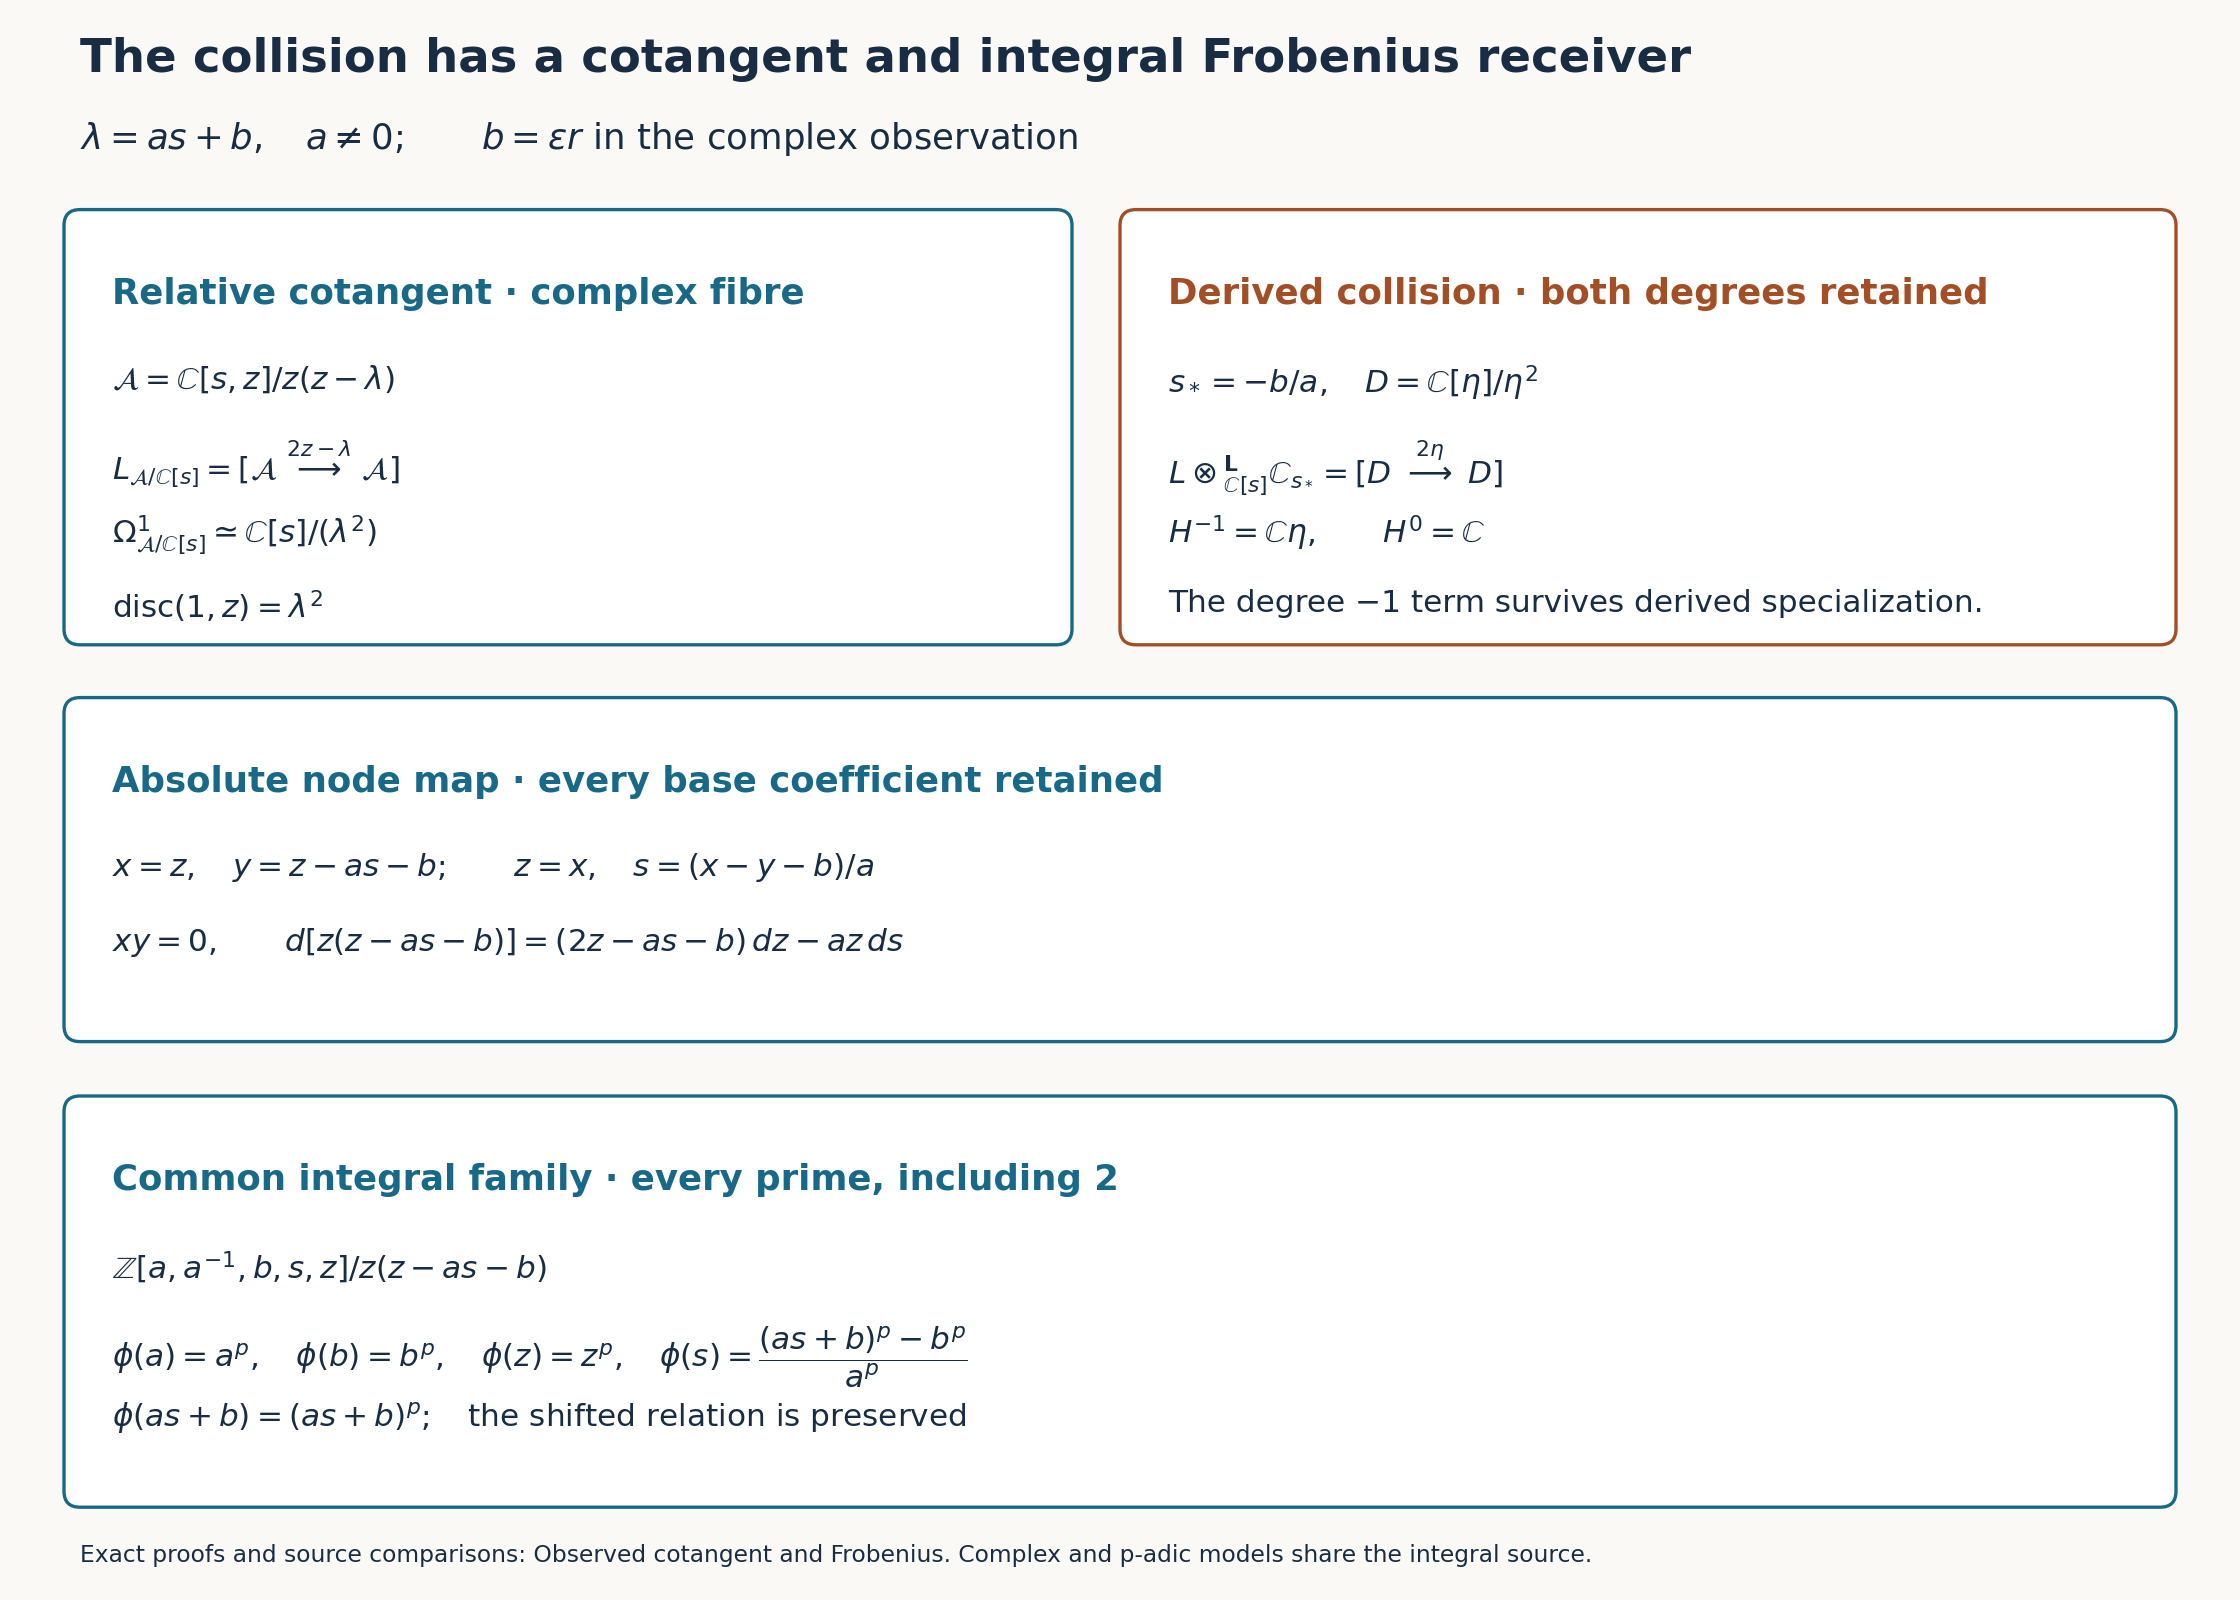
\includegraphics[keepaspectratio,alt={Relative and absolute cotangent maps, derived collision and integral Frobenius}]{figures/20_observed_cotangent.png}}
\caption{Relative and absolute cotangent maps, derived collision and
integral Frobenius}
\end{figure}

The diagram shows the complex cotangent and derived-fibre calculations
OCF4--OCF20 and the common integral source with corrected lift
OIF1--OIF11. In the lower panel the symbol b is the formal coefficient
called mathsf b in the text; in the complex specialization it maps to
epsilon r. The exact prime-2 torsion and divided map are OIF18--OIF19.
The diagram uses formulas rather than a sampled arithmetic period.

\end{document}
